\section{Language\label{sec:language}}

This section describes the \emph{dt} language in 
detail.  The section is divided into discussions of 
the high-level organization of a \emph{dt} program, 
the syntax of the language, and the code emitted by 
high-level language constructs.  There are also 
several code examples to highlight the flexibility 
of \emph{dt}.

\subsection{DT Program Organization}

Figure~\ref{pic:program} shows the high-level organization of a \emph{dt} program.
Each \emph{dt} program is composed of one or more mem() blocks.
The mem() blocks are used to encompass zero or more instructions, 
data values, and/or high-level language constructs.  A mem() block 
must be supplied with a starting address. Thus, multiple 
memory regions can be populated without the need to specify 
values in the memory "gaps". Each instruction will 
use 8 bytes of memory, in program order, starting from the mem() block
starting address.  Each data value put in the program source will 
use 4 bytes of memory.  If an instruction address is impacted
by a data value, the instruction's address will 
be aligned to the next 8 byte boundary. 

A single \emph{dt} program can be split into multiple files. 
By convention, those files are named with an extension of .dt. There 
are no restrictions on the number of mem() blocks or their 
locations for a program targeted for the flat memory of 
FabScalar cores.  The scratchpad memories of the debug core, on 
the other hand, come with a requirement of two mem() blocks. 
The debug core has two memories, with separate address spaces.
When emitting code for the scratchpads, you must use starting 
addresses of \texttt{0x0000} for the instruction scratchpad, and \texttt{0x1000}
for the data scratchpad.  Also, the data scratchpad cannot contain
instructions, only values.


\begin{figure}
\centering
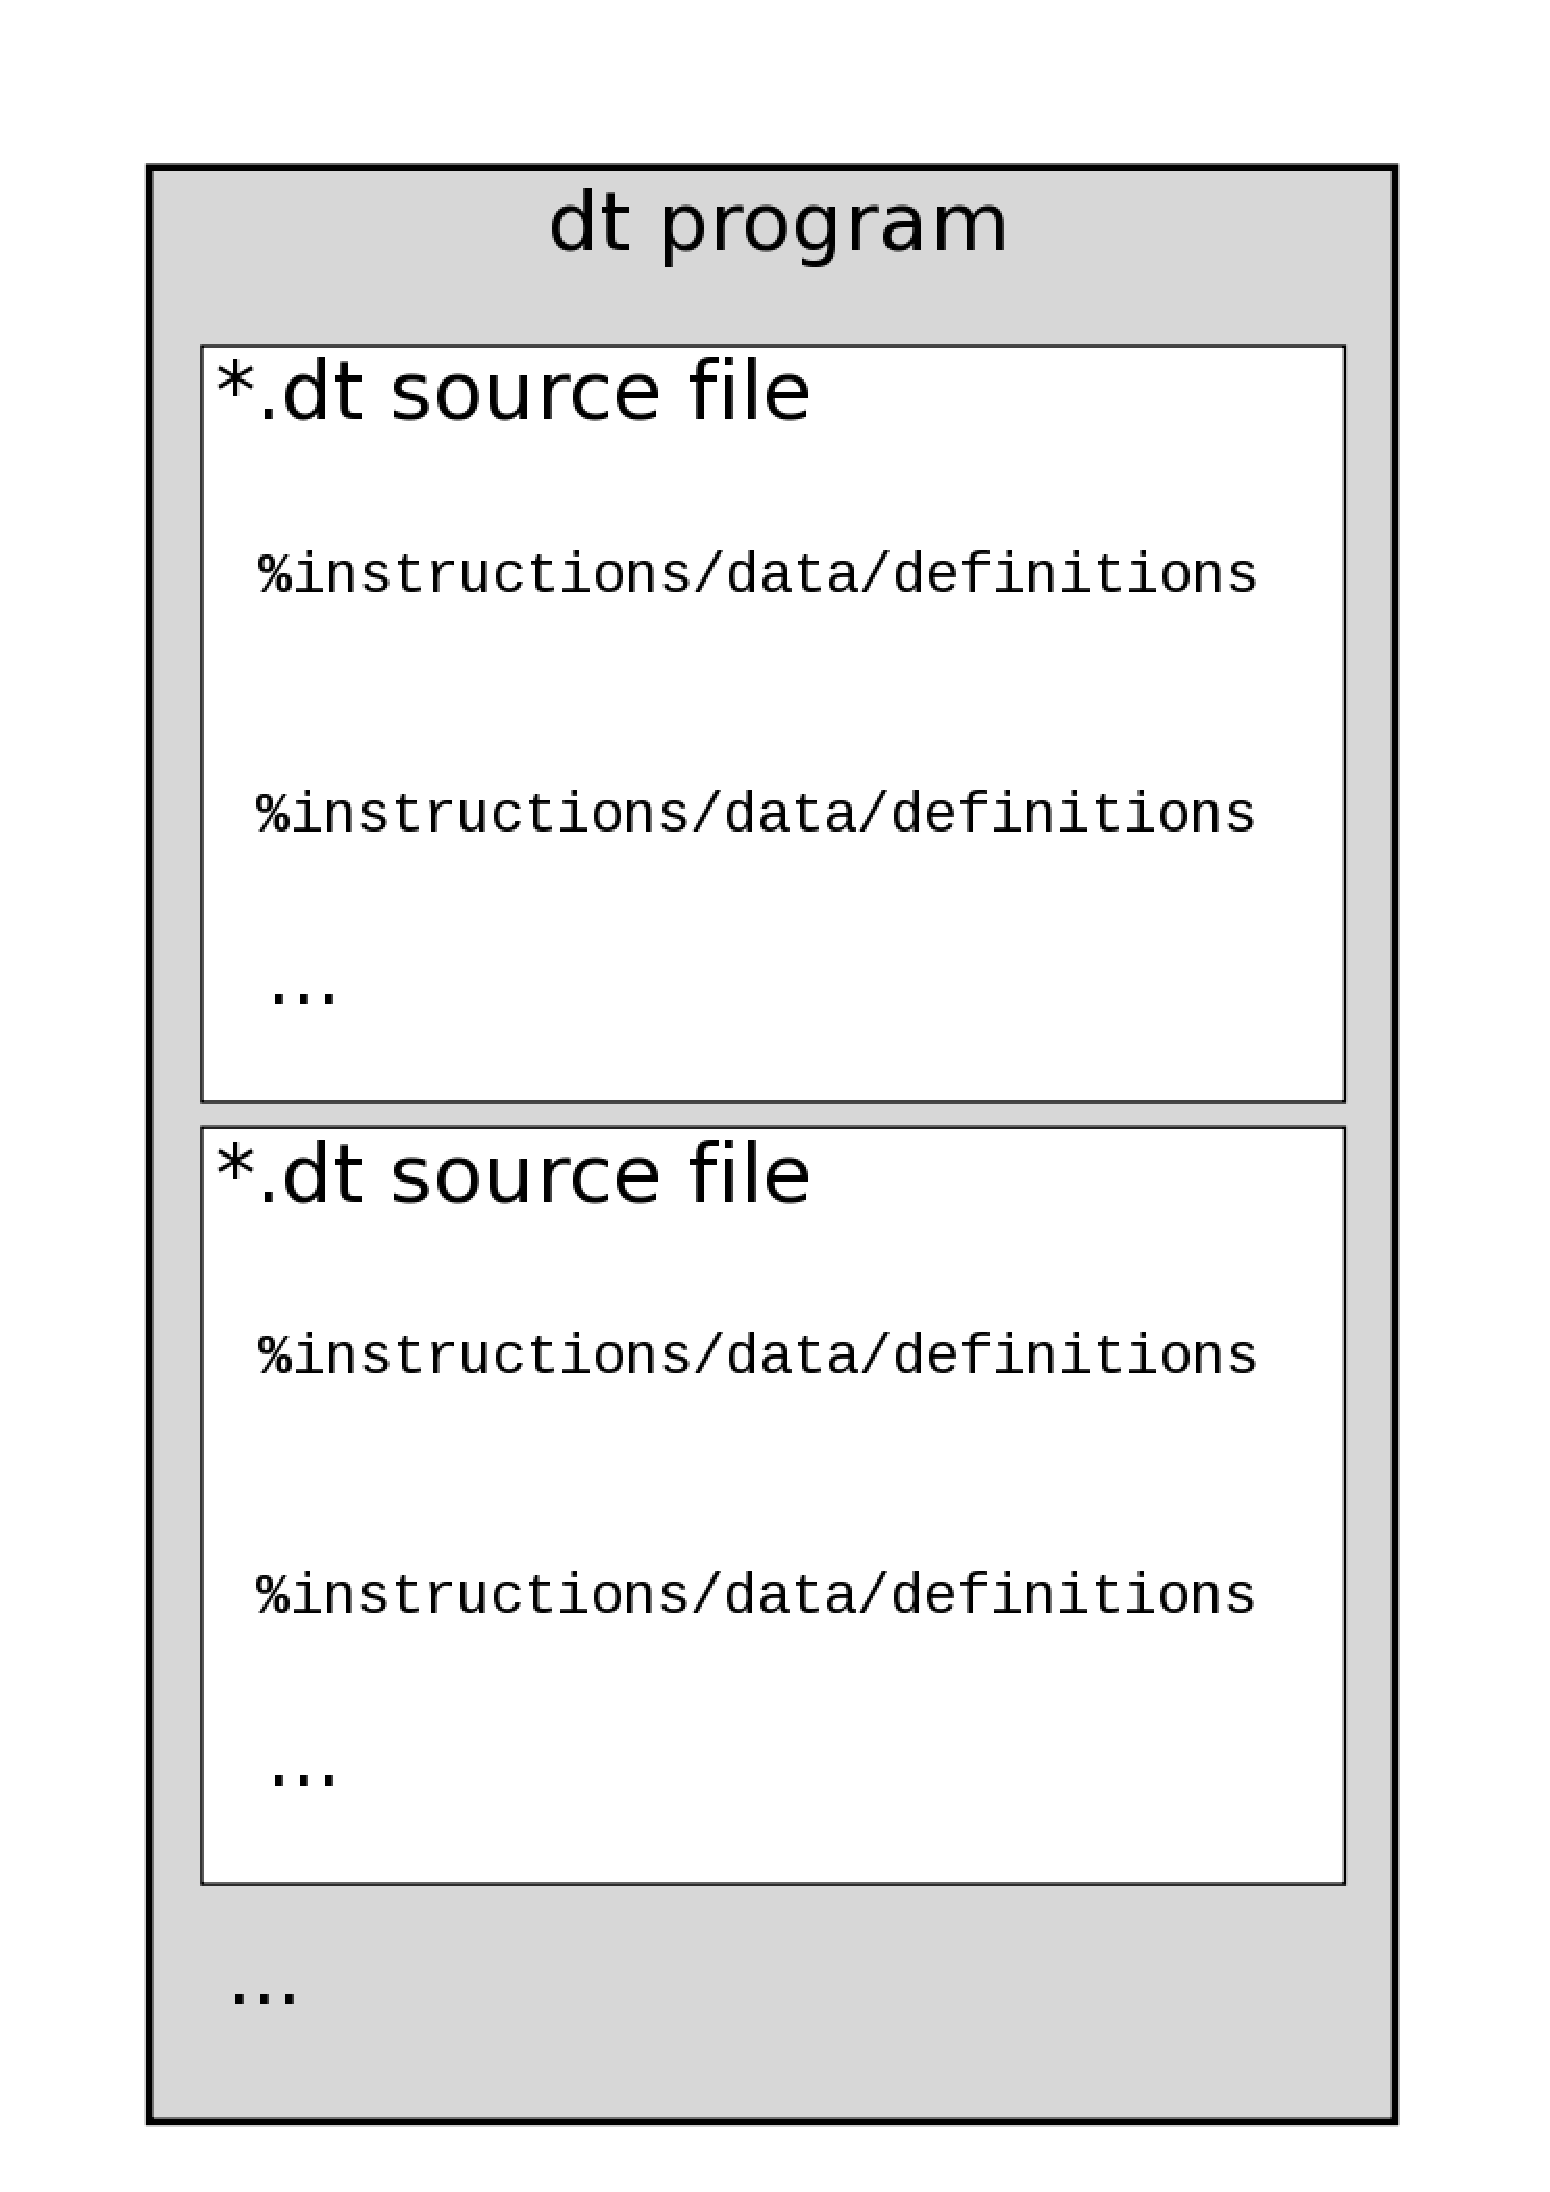
\includegraphics[width=0.45\textwidth]{figs/dt-program.pdf}
\caption{Program organization of a complete \emph{dt} program.}
\label{pic:program}
\vspace{-1em}
\end{figure}


%Describe the syntax and tricks of the language.  Think of 
%it as having two ways to write code (which can be intermixed) 
%like verilog: structural (asm statements) and behavioral (high-
%level constructs).

\subsection{Syntax}

The syntax of the \emph{dt} language can be sub-divided into
several categories: comments, mem() blocks, definitions, instructions, 
data values, high-level assignments, and high-level block statements.
White-space and linefeeds are ignored by the \emph{dt} 
compiler. Also, and very importantly, \emph{dt} is case-\textbf{sensitive} 
for definitions (section~\ref{sec:definitions}), but case-\textbf{insensitive} 
for all other constructs.

\subsubsection{Comments}

Comments can appear anywhere in the source file.  They start 
with a percent sign (\%) and extend to the remainder of the source line.
Multi-line comments are not allowed in \emph{dt}.  An example comment 
is shown in Listing~\ref{code:comment}.

\begin{lstlisting}[label=code:comment,caption=Code example of a comment,basicstyle=\footnotesize,numbers=left,numberstyle=\tiny,stepnumber=1, numbersep=6pt,frame=single,captionpos=b,escapechar=@]
% This is a comment.
\end{lstlisting}

\subsubsection{mem() Blocks}

A collection of any other syntatical construct other 
than comments must be contained within a mem() block.  
A mem() block indicates to the \emph{dt} compiler where
in the memory space the code contained within the mem() block
will be put.  That, in turn, impacts instruction and data
addresses, which themselves impact instruction offsets.

A mem() block is specified by the keyword \texttt{mem}. After 
the \texttt{mem} keyword, the starting address should be specified
within parenthesis.  The starting address should be formatted the 
same way as integer values as specified in section~\ref{sec:values}.
After the parenthesized starting address, the instructions and data of 
a mem() block 
should be encompassed in curly braces.  An example of a mem() 
block, with a starting address of \texttt{0x00400000}, is shown 
in Listing~\ref{code:memblock}.

\begin{lstlisting}[label=code:memblock,caption=Code example of a mem() block,basicstyle=\footnotesize,numbers=left,numberstyle=\tiny,stepnumber=1, numbersep=6pt,frame=single,captionpos=b,escapechar=@]
mem (0x00400000) {
% instructions, et. al., should go here 
}
\end{lstlisting}

\subsubsection{Definitions\label{sec:definitions}}

Definitions allow the programmer to name several of the
other \emph{dt} programming constructs.  A definition is 
a label followed by a colon follow by one of those 
program constructs.  A label can be any alpha-numeric 
string that starting with a letter.  The label can 
contain underscores (\_), but no other punctuation is 
allowed.  Remember that definitions are the only 
part of \emph{dt} that is  case-sensitive, 
so \texttt{label} is the different than \texttt{Label} is the 
different as \texttt{LABEL}.  There is no restriction on 
the length of the label.

There are two classes of definitions, those that 
name an associated memory location, and those that
name a register.  Registers are of the form: \texttt{\$r0-\$r31},
\texttt{\$hi}, and \texttt{\$lo} for the integer registers. 
Once a register is given a name, the instructions that follow
can then refer to the name in place of the register number.
A named memory location can be used by other instructions
to assist in forming addresses, or in leaving offset
calculations to the compiler. 

The floating point registers \texttt{\$f0-\$f31}, and 
\texttt{\$t0-\$t31} for the Teleport Register File (TRF) registers
are available in the language for instructions, but cannot be 
named using a definition.

Note that all definitions are global.  Also note that 
registers must be named with a register definition
before that label can be used by any instructions, 
but memory definitions can come in any order.
Registers can be renamed as often as needed, 
memory locations can typically only be labeled once
except for rare circumstances. Since labels are 
global, it is possible to refer to registers
and/or memory locations that span different mem() blocks.
Listing~\ref{code:definitions} shows two example 
definitions, one for a register, and another to 
name a memory location that holds an \texttt{ADDI} instruction.
Since the ADDI instruction is the first (and only)
element that requires a memory location, 
\texttt{bar} is naming memory location \texttt{0x00400000}.

\begin{lstlisting}[label=code:definitions,caption=Code example of a register and memory definition,basicstyle=\footnotesize,numbers=left,numberstyle=\tiny,stepnumber=1, numbersep=6pt,frame=single,captionpos=b,escapechar=@]
mem (0x00400000) {
    foo: $r5  % gives $r5 a handy name
    bar: addi foo, $r0, 0x7
}
\end{lstlisting}

\subsubsection{Data and Immediate Values\label{sec:values}}

Values are used in two main ways in \emph{dt} programs. Some
instructions require immediate values or offsets.  Alternatively, 
it is possible to simply initialize a memory location with 
a known value.

Integer values can be specified in either decimal or hexadecimal.
To indicate a decimal value, use a hash (\texttt{\#}) followed 
by an optional sign (\texttt{+} or \texttt{-}), followed by the
numerical value. A hexadecimal value is specified exactly the 
same way as in the C programming language -- a \texttt{0x} followed
by the hexadecimal value.  Listing~\ref{code:values}, line 2 shows an ADDI
instruction, where the immediate has the value -1. Values 
used for immediates and offsets are 
still bound by the number of bits in the instruction encodings.
Floating point values are also possible. They are denoted in a similar way 
as in the C programming language with an optional sign, a whole value,
a decimal point, a fractional value, and an optional exponent which is
denoted with the letter \texttt{e}, an optional sign, and the value of 
the exponent.  The difference with with C is that floating point values 
in \emph{dt} must be preceeded with a hash.

\begin{lstlisting}[label=code:values,caption=Code example of immediate values and initialized memory locations,basicstyle=\footnotesize,numbers=left,numberstyle=\tiny,stepnumber=1, numbersep=6pt,frame=single,captionpos=b,escapechar=@]
mem (0x00400000) {
    addi $r1, $r0, #-1
    ! 0xdeadbeef
    ! #2.998e8
}
\end{lstlisting}

Memory can be initialized with a starting value.  The syntax 
to fill a memory location is to use a bang (\texttt{!}), then 
list the value thereafter.  Listing~\ref{code:values}, line 3 
initializes location \texttt{0x00400008} with the value \texttt{0xdeadbeef}, 
and line 4 initializes location \texttt{0x0040000c} with 
the 32 bit IEEE encoded floating point value for $2.998\times10^8$.

\subsubsection{Instructions}

Instructions can be specified by the usual instruction
mnemonics, following the syntax in the PISA ISA specification~\cite{burger97}.
Some instructions have alternative forms that will be 
discussed in section~\ref{sec:assign}.  Table~\ref{tab:opcodes}
lists the valid opcodes that can be used.

\begin{table}
\centering
\caption{Instruction opcodes recognized by the \emph{dt} compiler}
\begin{tabular}{|l|l|l|l|l|}
\hline
\textbf{Arithmetic} & \textbf{Memory} & \textbf{CTI} & \textbf{FP} & \textbf{Other} \\ \hline \hline
add & lb & j & add.s & nop \\ \hline
addi & lbu & jal & add.d & syscall \\ \hline
addu & lh & jr & sub.s & break \\ \hline
addiu & lhu & jalr & sub.d & mfc1 \\ \hline
sub & lw & beq & mul.s & mtc1 \\ \hline
subu & dlw & bne & mul.d & m1t\_trf \\ \hline
mult & l.s & blez & div.s & m2t\_trf \\ \hline
multu & l.d & bgtz & div.d & mf\_trf \\ \hline
div & lwl & bltz & abs.s & barrier \\ \hline
divu & lwr & bgez & abs.d & eret \\ \hline
mfhi & sb & bc1f & mov.s & migrate \\ \hline
mthi & sh & bc1t & mov.d &  \\ \hline
mflo & sw & return & neg.s &  \\ \hline
mtlo & dsw & & neg.d &  \\ \hline
and & dsz & & cvt.s.d &  \\ \hline
andi & s.s & & cvt.s.w &  \\ \hline
or & s.d & & cvt.d.s &  \\ \hline
ori & swl & & cvt.d.w &  \\ \hline
xor & swr & & cvt.w.s &  \\ \hline
xori & & & cvt.w.d &  \\ \hline
nor & & & c.eq.s &  \\ \hline
sll & & & c.eq.d &  \\ \hline
sllv & & & c.lt.s &  \\ \hline
srl & & & c.lt.d &  \\ \hline
srlv & & & c.le.s &  \\ \hline
sra & & & c.le.d &  \\ \hline
srav & & & sqrt.s &  \\ \hline
slt & & & sqrt.d &  \\ \hline
slti & & & &  \\ \hline
sltu & & & &  \\ \hline
sltiu & & & &  \\ \hline
lui & & & &  \\ \hline
\end{tabular}
\label{tab:opcodes}
\end{table}

Listing~\ref{code:insts} gives examples 
of several types of instructions.  Instructions are 
fully specified using their opcode, followed by 
their operands.  Operands can be specified in several ways, depending
on the instruction type.  For instructions with all register operands,
typically the destination register is listed first, followed by the 
source operands.  This is the typical format for arithmetic and logical 
instructions.  In the example code Listing~\ref{code:insts}, line 
2 shows an example ADD instruction with source registers \texttt{\$r0} and 
\texttt{\$r3} and destination register \texttt{\$r5}.  Note that the MULT
and DIV instructions (and their variants) have an implied destination register 
of \texttt{\$hi} and \texttt{\$lo}, these should not be listed 
when using the MULT and DIV instructions -- only the source 
operands are needed.

Memory instructions can follow a similar form as arithmetic operations,
with a list of registers and/or offsets.  Loads have their destination 
register listed first, followed by the address register(s), followed 
by an offset if necessary.  Stores should list their data operand register
first, followed by the address register(s) and offset.  However, loads and 
stores have an alternative format in which the address register is surrounded 
with parantheses, and the offset or offset register is listed before the
parantheses. This syntax is similar to the form seen in the PISA ISA document
and in assembly dumps.  Listing~\ref{code:insts} line 3 shows an example of this 
alternate syntax.  In that example, the address in register \texttt{\$r5} is 
added to the offset of 0, and the value at that location is written to
destination register \texttt{\$r9}.

\begin{lstlisting}[label=code:insts,caption=Code example of several instructions,basicstyle=\footnotesize,numbers=left,numberstyle=\tiny,stepnumber=1, numbersep=6pt,frame=single,captionpos=b,escapechar=@]
mem (0x00400000) {
        add $r5, $r0, $r3
        lw $r9, #0($r5)
        bltz $r9, target
        % some code
target: nop
}
\end{lstlisting}

Control transfer instructions have no destination register, so their 
source register(s), if any, are listed immediately after the opcode.
For the instructions that allow for direct targets (either immediate 
addresses, or offsets from the PC), the \emph{dt} compiler allows 
you to use a labeled memory location in place of the offset.  In that
case, the compiler will determine the appropriate address or offset
automatically.  Listing~\ref{code:insts} line 4 shows that a BLTZ
instruction will skip over some code to a NOP named target if the BLTZ 
is taken.  Table~\ref{tab:opcodes} lists a RETURN instruction, which 
is a pseudo-op for a JR instruction with register \texttt{\$r31}. The
RETURN, if used, requires no operands.

There are several instructions listed for Fast Thread Migration.  The
move instructions to/from the TRF will always use the same register 
number when copying registers.  That is, copying \texttt{\$r1} to
the TRF implies that \texttt{\$r1} is copied to \texttt{\$t1}.  The
BARRIER, ERET, and MIGRATE instructions have no operands.

\subsubsection{Assignments\label{sec:assign}}

Many common operations have an alternative shorthand notation 
which is similar to the C set of operations.  The general form 
is to list a destination register (or named register), followed 
by one of the operands and operators listed in Table~\ref{tab:operators}.
Note that only a single operation can be done per assignment,
compound operations, or operations on three or more operands
are not allowed.  This is because the \emph{dt} compiler
does not do register allocation.  So, the programmer
must use separate lines for each intermediate result.

\begin{table}
\centering
\caption{Assignment operations allowed by the \emph{dt} compiler}
\begin{tabular}{|l|l|}
\hline
\textbf{Operation Format} & \textbf{Resulting Instruction} \\ \hline \hline
\emph{\textless ireg\textgreater} = \emph{\textless ireg\textgreater} + \emph{\textless ireg\textgreater} & ADD \\ \hline
\emph{\textless ireg\textgreater} = \emph{\textless ireg\textgreater} + \emph{\textless imm\textgreater} & ADDI \\ \hline
\emph{\textless ireg\textgreater} = \emph{\textless ireg\textgreater} - \emph{\textless ireg\textgreater} & SUB \\ \hline
\emph{\textless ireg\textgreater} = \emph{\textless ireg\textgreater} - \emph{\textless imm\textgreater} & SUBI \\ \hline
\emph{\textless reglo\textgreater} = \emph{\textless ireg\textgreater} * \emph{\textless imm\textgreater} & MULT \\ \hline
\emph{\textless reglo\textgreater} = \emph{\textless ireg\textgreater} / \emph{\textless imm\textgreater} & DIV \\ \hline
\emph{\textless ireg\textgreater} = \emph{\textless ireg\textgreater} & See discussion \\ \hline
\emph{\textless ireg\textgreater} = \emph{\textless imm\textgreater} & See discussion \\ \hline
\emph{\textless ireg\textgreater} = -\emph{\textless ireg\textgreater} & SUB \\ \hline
\emph{\textless ireg\textgreater} = \emph{\textless ireg\textgreater} \& \emph{\textless ireg\textgreater} & AND \\ \hline
\emph{\textless ireg\textgreater} = \emph{\textless ireg\textgreater} \& \emph{\textless imm\textgreater} & ANDI \\ \hline
\emph{\textless ireg\textgreater} = \emph{\textless ireg\textgreater} $\vert$ \emph{\textless ireg\textgreater} & OR \\ \hline
\emph{\textless ireg\textgreater} = \emph{\textless ireg\textgreater} $\vert$ \emph{\textless imm\textgreater} & ORI \\ \hline
\emph{\textless ireg\textgreater} = \emph{\textless ireg\textgreater} \textasciicircum \emph{\textless ireg\textgreater} & XOR \\ \hline
\emph{\textless ireg\textgreater} = \emph{\textless ireg\textgreater} \textasciicircum \emph{\textless imm\textgreater} & XORI \\ \hline
\emph{\textless ireg\textgreater} = ~\emph{\textless ireg\textgreater} & NOR (performs bitwise NOT) \\ \hline
\emph{\textless ireg\textgreater} = ~\emph{\textless imm\textgreater} & See discussion \\ \hline
\emph{\textless ireg\textgreater} = \emph{\textless ireg\textgreater} $<<$ \emph{\textless imm\textgreater} & SLL \\ \hline
\emph{\textless ireg\textgreater} = \emph{\textless ireg\textgreater} $<<$ \emph{\textless ireg\textgreater} & SLLV \\ \hline
\emph{\textless ireg\textgreater} = \emph{\textless ireg\textgreater} $>>$ \emph{\textless imm\textgreater} & SRL \\ \hline
\emph{\textless ireg\textgreater} = \emph{\textless ireg\textgreater} $>>$ \emph{\textless ireg\textgreater} & SRLV \\ \hline
\emph{\textless ireg\textgreater} = \emph{\textless ireg\textgreater} $<$ \emph{\textless ireg\textgreater} & SLT \\ \hline
\emph{\textless ireg\textgreater} = \emph{\textless ireg\textgreater} $<$ \emph{\textless imm\textgreater} & SLTI \\ \hline
\emph{\textless ireg\textgreater} = \emph{\textless ireg\textgreater} $>$ \emph{\textless ireg\textgreater} & Not yet implemented \\ \hline
\emph{\textless ireg\textgreater} = \emph{\textless ireg\textgreater} $>$ \emph{\textless imm\textgreater} & Not yet implemented \\ \hline
\emph{\textless ireg\textgreater} = \emph{\textless ireg\textgreater} $<$= \emph{\textless ireg\textgreater} & Not yet implemented \\ \hline
\emph{\textless ireg\textgreater} = \emph{\textless ireg\textgreater} $<$= \emph{\textless imm\textgreater} & Not yet implemented \\ \hline
\emph{\textless ireg\textgreater} = \emph{\textless ireg\textgreater} $>$= \emph{\textless ireg\textgreater} & Not yet implemented \\ \hline
\emph{\textless ireg\textgreater} = \emph{\textless ireg\textgreater} $>$= \emph{\textless imm\textgreater} & Not yet implemented \\ \hline
\emph{\textless ireg\textgreater} = \emph{\textless ireg\textgreater} == \emph{\textless ireg\textgreater} & Not yet implemented \\ \hline
\emph{\textless ireg\textgreater} = \emph{\textless ireg\textgreater} == \emph{\textless imm\textgreater} & Not yet implemented \\ \hline
\emph{\textless ireg\textgreater} = \emph{\textless ireg\textgreater} != \emph{\textless ireg\textgreater} & Not yet implemented \\ \hline
\emph{\textless ireg\textgreater} = \emph{\textless ireg\textgreater} != \emph{\textless imm\textgreater} & Not yet implemented \\ \hline
\emph{\textless ireg\textgreater} = @\emph{\textless label\textgreater} & LUI, ADDI (address-of) \\ \hline
\emph{\textless freg\textgreater} = \emph{\textless freg\textgreater} + \emph{\textless freg\textgreater} & ADD.S \\ \hline
\emph{\textless freg\textgreater} = \emph{\textless freg\textgreater} - \emph{\textless freg\textgreater} & SUB.S \\ \hline
\emph{\textless freg\textgreater} = \emph{\textless freg\textgreater} * \emph{\textless freg\textgreater} & MUL.S \\ \hline
\emph{\textless freg\textgreater} = \emph{\textless freg\textgreater} / \emph{\textless freg\textgreater} & DIV.S \\ \hline
\emph{\textless freg\textgreater} = \emph{\textless freg\textgreater} & MOV.S \\ \hline
\emph{\textless freg\textgreater} = -\emph{\textless freg\textgreater} & NEG.S \\ \hline
\end{tabular}
\label{tab:operators}
\end{table}

Some operations listed in Table~\ref{tab:operators} require more
than one instruction, or require one of many possible different 
instructions.  Assigning an integer register to another integer 
register is simply a case of using an ADDI with zero immediate to 
do the copy, unless one of the registers is \texttt{\$hi} or \texttt{\$lo}.
In that case, the appropriate MTHI, MFHI, MTLO, or MFLO is used.
Also, when assigning an immediate value to a register, depending 
on the size of the immediate, the operation may be done with 
a single ADDI, or may require an LUI followed by an ADDI. This 
is also the case when performing the bitwise NOT of an immediate.

Several of the comparison operators have not yet been implemented.
This is because PISA does not have single instructions to 
perform the comparison.  These operations will require several 
instructions each, and is left for future work.

Listing~\ref{code:assign} shows two mem() blocks with equivalent 
instructions.  However, one mem() block is written using the 
instruction mnemonics, and the other is written using the 
shorthand assignments.  These two mem() blocks will produce binary
equivalent instructions.  Note that these mem() blocks could not 
appear in the same program, as their memory regions would overlap.

\begin{lstlisting}[label=code:assign,caption=Code example of equivalent instructions using (a) instruction mnemonics and (b) shorthand assignments,basicstyle=\footnotesize,numbers=left,numberstyle=\tiny,stepnumber=1, numbersep=6pt,frame=single,captionpos=b,escapechar=@]
% code block (a)
mem (0x00400000) {
    addi $r1, $r0, #3
    nor  $r1, $r1, $r1
    and  $r3, $r2, $r1
    slt  $r4, $r3, $r0
}

% code block (b)
mem (0x00400000) {
zero: $r0
mask: $r1
val:  $r2
res:  $r3
cond: $r4

      mask = #3
      mask = ~mask
      res = val & mask
      cond = res < zero
}
\end{lstlisting}

\subsubsection{Block Statements}

The last group of syntatical constructs provide the 
high-level language-like features of if-statements and loops.
The syntax for each of these constructs is similar 
to the C programming language.  However, the major 
difference is that the condition must be a single 
register or named register.  This is because a complex
condition requires a temporary register, and the \emph{dt}
compiler does not do register allocation.  This also 
eliminates the \texttt{for} loop from availability: the 
initial value, and increment amount could be handled, 
but the comparison to know when the loop should stop 
requires a register.  The \emph{dt} compiler also 
has no formal mechanism or syntatical construct for 
functions.  This is due to the several requirements 
that functions require, a runtime stack, the stack pointer, 
the return register, function arguments, and so on -- all of 
these are against the intent behind \emph{dt} to give 
all control to the programmer.

The constructs that are available however, are: if-statements,
if-else statements, while loops, do...while loops, until loops,
and do...until loops.  These constructs can contain instructions,
definitions, values (if you really want to mix instructions with
data), assignments, and other block statements.  These block 
statements can also be named themselves -- simply provide a 
label followed by a colon followed by the block statement.  This 
will name the first instruction of the block statement. That named instruction 
might be an instruction in the body of the block statement as 
in do...while and do...until loops, or it might be an 
instruction that is not evident in the code (i.e. part of the 
supporting code emitted by the block statement).

The condition for each of the statements must be an 
integer register or label that corresponds to an integer 
register.  The meaning, however, is the same as in C -- 
any non-zero value is considered \texttt{true}, and zero 
is considered \texttt{false}.  Table~\ref{tab:blocks} gives 
the syntax for each of the constructs and the code generated 
by the \emph{dt} compiler.

\begin{table}
\centering
\caption{High-level code blocks recognized by the \emph{dt} compiler}
\begin{tabular}{|l|}
\hline
\textbf{Syntax} \\ \hline \hline
if (\emph{\textless ireg\textgreater}) \{ \\
\% instructions, code blocks here \\
\} \\ \hline
if (\emph{\textless ireg\textgreater}) \{ \\
\% instructions, code blocks here \\
\} \\
else \{ \\
\% instructions, code blocks here \\
\} \\ \hline
while (\emph{\textless ireg\textgreater}) \{ \\
\% instructions, code blocks here \\
\} \\ \hline
until (\emph{\textless ireg\textgreater}) \{ \\
\% instructions, code blocks here \\
\} \\ \hline
do \{ \\
\% instructions, code blocks here \\
\} while (\emph{\textless ireg\textgreater}) \\ \hline
do \{ \\
\% instructions, code blocks here \\
\} until (\emph{\textless ireg\textgreater}) \\ \hline
\end{tabular}
\label{tab:blocks}
\end{table}

TODO: The emitted code for each of these constructs.

\subsection{Code Examples}

This section includes a handful of example programs written in \emph{dt}.
The intent is to show full program examples, and also to show 
the flexibility of the syntax.

\subsubsection{Matrix Multiply}
The first program is used to compute a matrix multiplication of 
two matrices, call them \textbf{A} and \textbf{B}, and write the 
result to matrix \textbf{C}.  The matrices are
4 rows by 4 columns and their data is initialized in a 
separate mem() block from the instructions and are saved 
in row-major form as would have been done by a C compiler.  The code is 
shown in Listing~\ref{code:matmult}.


\begin{lstlisting}[label=code:matmult,caption=Matrix multiplication example source code,basicstyle=\footnotesize,numbers=left,numberstyle=\tiny,stepnumber=1, numbersep=6pt,frame=single,captionpos=b,escapechar=`]
$pc = 0x00400000

mem (0x00400000) {
ii:      $r1
jj:      $r2
kk:      $r3
icond:   $r4
jcond:   $r5
kcond:   $r6
aaddr:   $r7
baddr:   $r8
caddr:   $r9
aval:    $r10
bval:    $r11
cval:    $r12
mtemp:   $r13
stemp:   $r14
four:    $r15
sixteen: $r16
mres:    $lo

    four = #4
    sixteen = #16
    ii = #0
    icond = ii < #4
    while (icond) {
        jj = #0
        jcond = jj < #4
        while (jcond) {
            % initialize c[i][j] to zero
            cval = #0

            kk = #0
            kcond = kk < #4
            while (kcond) {
                % compute address of a[i][k]
                aaddr = @A
                mres = ii * sixteen
                mtemp = mres
                mres = kk * four
                stemp = mres
                mtemp = mtemp + stemp
                aaddr = aaddr + mtemp

                % compute address of a[k][j]
                baddr = @B
                mres = kk * sixteen
                mtemp = mres
                mres = jj * four
                stemp = mres
                mtemp = mtemp + stemp
                baddr = baddr + mtemp

                % load the values of a[i][k] and b[k][j]
                lw aval, #0[aaddr]
                lw bval, #0[baddr]

                % c[i][j] += a[i][k] * b[k][j]
                mres = aval * bval
                mtemp = mres
                cval = cval + mtemp

                kk = kk + #1
                kcond = kk < #4
            }

            % compute c[i][j] address
            caddr = @C
            mres = ii * sixteen
            mtemp = mres
            mres = jj * four
            stemp = mres
            mtemp = mtemp + stemp
            caddr = caddr + mtemp

            % store c[i][j]
            sw cval, #0[caddr]

            jj = jj + #1
            jcond = jj < #4
        }
        ii = ii + #1
        icond = ii < #4
    }
}

% matrix data
mem (0x10000000) {
A : ! #10
    ! #2
    ! #7
    ! #-4
    ! #9
    ! #-2
    ! #12
    ! #1
    ! #17
    ! #8
    ! #-3
    ! #1
    ! #6
    ! #-5
    ! #13
    ! #0

B : ! #3
    ! #7
    ! #9
    ! #-2
    ! #15
    ! #-1
    ! #4
    ! #6
    ! #11
    ! #8
    ! #3
    ! #-7
    ! #1
    ! #10
    ! #4
    ! #-5

C : ! #0
}
\end{lstlisting}

\subsubsection{Pseudo-Function}

This example defines a type of function that is called from a 
main program.  The function semantics are passing all values
through registers, so no runtime stack is defined.
